\section{Exercise 4: Matrix-Matrix-Multiplication I}
\begin{frame}[fragile]
\frametitle{Memory access}
Relevant code:
\codestylec
\begin{lstlisting}
    for(i = 0; i < n; i++){
        for(j = 0; j < n; j++){
            for(k = 0; k < n; k++){
                c[i * n + j] += a[i * n + k] * b[k * n + j];
            }
        }
    }
\end{lstlisting}
Observations:
\begin{itemize}
\item Access to c constant within loop
\item Access to a with unit-stride
\item Access to b with stride n
\end{itemize}

\end{frame}

\begin{frame}{Compiler-Directives}
\begin{itemize}
\item compiler option -O3
	\begin{itemize}
	\item Automatic vectorization
	\item Advanced loop transformation 
	\end{itemize}
\item pragma vector aligned
	\begin{itemize}
	\item use \texttt{memalign()} instead of \texttt{malloc()}
	\item \texttt{\#pragma vector aligned} before the innermost loop
	\end{itemize}
\end{itemize}
\end{frame}

\begin{frame}{MFLOPS and cache-miss rates}
\begin{figure}[h]
  \begin{center}
    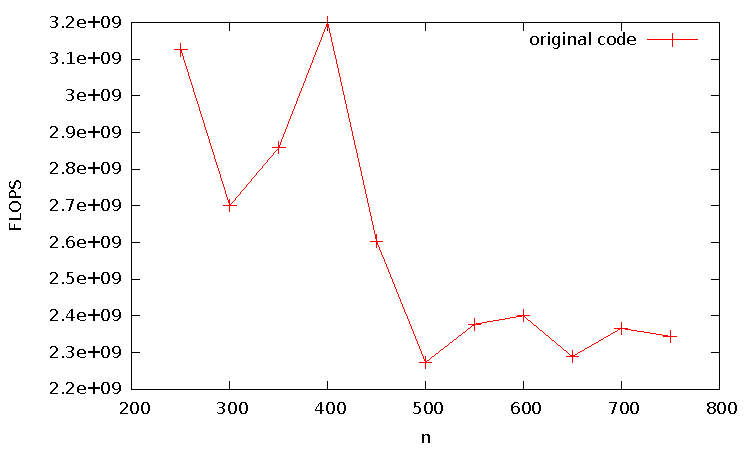
\includegraphics[width=0.9\textwidth]{../graphics/graph_unblocked.pdf}
    %\caption{Results of non-blocked matrix multiplication}
  \end{center}
\end{figure}
\begin{itemize}
\item Best performance for n = 400
\item Performance is not stable
\item For n $>$ 500: cache-inefficient
\end{itemize}
\end{frame}

\begin{frame}{The effect of compiler options}
\begin{itemize}
\item From -O0 to -O1: factor of three
\item From -O0 to -O2: factor of ten
\item From -O2 to -O3: No noticeably difference
\item From -O2 to -fast: factor of 1.5
\end{itemize}
\end{frame}

\begin{frame}[fragile]
\frametitle{Cache-blocking: Code}
\codestylec
\begin{lstlisting}
for(ii=0; ii<n; ii+=blockSize){
for(jj=0; jj<n; jj+=blockSize){
for(kk=0; kk<n; kk+=blockSize){
    for(i=0; i<blockSize && ii+i<n; ++i){
        for(j=0; j<blockSize && jj+j<n; ++j){
            int const kStop = mymin(blockSize, n-kk);
            s = c[(ii + i)*n + jj + j];
#pragma vector aligned
            for(k=0; k<kStop; ++k){
                s += a[(ii + i)*n + kk + k] * 
                     b[(kk + k)*n + jj + j];
            }
            c[(ii + i)*n + jj + j] = s;
        }
    }
}
}
}
\end{lstlisting}
\end{frame}

\begin{frame}{Cache-blocking: Effect}
\begin{figure}[h]
  \begin{center}
    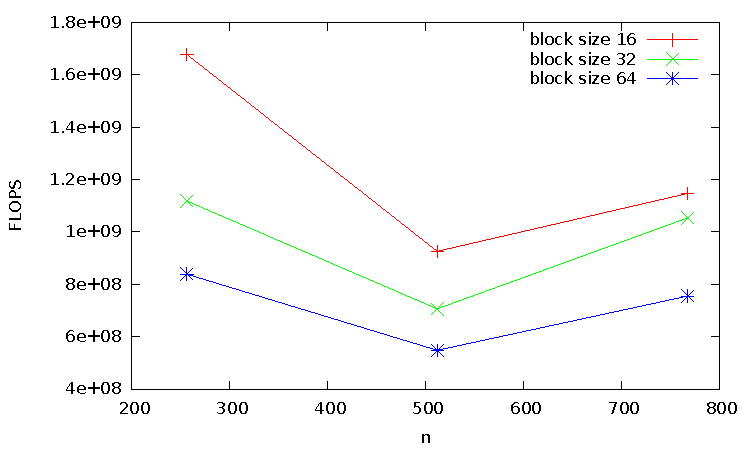
\includegraphics[width=0.9\textwidth]{../graphics/graph_blocked_flops.pdf}
  \end{center}
\end{figure}
\begin{itemize}
\item Lower MFLOPS rate than the non-blocked version
\end{itemize}
\end{frame}

\begin{frame}{Cache-blocking with vector intrinsics}
\begin{figure}[h]
  \begin{center}
    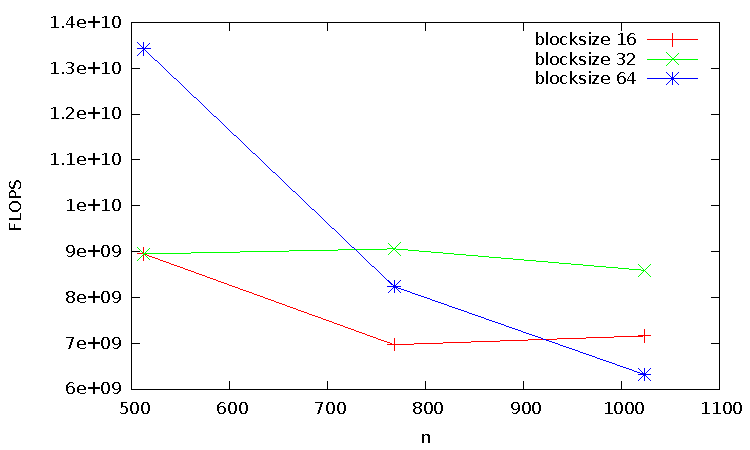
\includegraphics[width=0.9\textwidth]{../graphics/graph_avx.pdf}
  \end{center}
\end{figure}
\begin{itemize}
\item About 3x Higher MFLOPS rate than the non-blocked version
\end{itemize}
\end{frame}
